\chapter{State of the art}
\label{ch:stand-van-zaken}

Een moderne website wordt gemaakt met drie belangrijke technologieën: \gls{HTML} voor inhoud, \gls{CSS} voor vormgeving, en \gls{Javascript} om de pagina interactief te maken. Deze drie kunnen allemaal aan elkaar worden gekoppeld, ergens op een server worden gezet en dan kan een gebruiker een werkende website laden. Ook al zijn de grote web platformen van vandaag, zoals Facebook en Youtube, allemaal gebaseerd op deze technologieën, er zijn veel meer ingrediënten nodig om ze te laten werken.

Voor het maken van een simpele, statische site zijn de drie basistechnologieen van het web alles wat we nodig hebben. Het is echter een heel ander verhaal voor een ontwikkelaar die een complexere site wil maken, een reactieve site, een site die gebruik maakt van \gls{open-source} \gls{packages} of die gewoon zijn eigen werk wat makkelijker wil maken. Er zijn duizenden bibliotheken, packages en frameworks die webontwikkeling mogelijk maken op een heel nieuw niveau en eenvoudiger dan ooit tevoren \autocite{NPM}. Dit stelt ons echter voor een nieuw probleem. 

Als we een webapplicatie zouden maken met een enkel \gls{Javascript} bestand zonder afhankelijkheden i.e. geen andere bestanden die gelinkt zijn aan dat \gls{Javascript} bestand, het linken aan een index.html en tot slot wat \gls{CSS} toevoegen, zou die site prima werken. Maar wat als we een tweede \gls{Javascript} bestand introduceren en daar naar verwijzen in het andere bestand. Wat als we een \gls{open-source} \gls{package} willen installeren en gebruiken, gedownload van een \gls{package-manager} zoals NPM? Wat als we \gls{SASS} willen gebruiken om \gls{CSS} uit te breiden? Dit zou allemaal niet werken. De browser weet gewoon niet hoe alle verschillende stukjes aan elkaar te plakken.
We hebben iets nodig dat alle verschillende \gls{Javascript} bestanden en zijn afhankelijkheden bundelt, iets dat de \gls{SASS} bestanden begrijpt en correct laadt, of welk ander bestand dan ook. We hebben een module bundler nodig. In essentie, nemen zij alle verschillende bronbestanden in een project en bundelt die tot een enkel uitvoer bestand dat de browser begrijpt.

\section{Geschiedenis}

Om de rest van dit hoofdstuk te begrijpen, moet eerst een \gls{Javascript} module uitgelegd worden. Modulair programmeren splitst een programma op in brokken gebaseerd op functionaliteit en vaak in aparte bestanden. Deze brokken worden modules genoemd. Modules worden dan aan elkaar gekoppeld om een applicatie te vormen. \autocite{webpack-no-dateB} \autocite{mozilla-2021A}

Node.js, een runtime voor computers en servers waardoor \gls{Javascript} applicaties los van een browser kunnen draaien, ondersteunt modulair programmeren vanaf het begin met CommonJS. Ondersteuning voor modules in de browser daarentegen was niet bestaand. De eerste module bundlers kwamen pas na 2014. Om te begrijpen waarom module bundlers bestaan, moeten we eerst weten hoe webapplicaties voor hen werden gebouwd en welk probleem ze oplosten. \autocite{webpack-no-dateA}

\subsection{Script tags}

\gls{Javascript} kan worden gekoppeld aan, of direct worden geschreven in, het \gls{HTML}-bestand van een site met behulp van script-tags. Dit wetende, zouden wij een verschillende tag en corresponderend \gls{Javascript} bestand kunnen gebruiken voor elke toepassing van de applicatie. Laten we zeggen dat er een bestand is met alle code voor het aanmelden van een gebruiker en een ander voor algemene gebeurtenissen (op een knop klikken, \ldots). Dit is prima wanneer we slechts twee bestanden hebben die niet zo groot zijn, maar introduceert knelpunten voor het dataverkeer wanneer dit geschaald zou worden naar een grotere applicatie. Hetzelfde geldt als al de code in één groot bestand zou staan. Het globale domein van de browser zou ook vervuild raken met onze eigen functies. Aangezien sommige, of alle, functies beschikbaar zijn in het globale domein, zou dit veiligheidsrisico's en naam botsingen kunnen introduceren. 

\lstinputlisting[language=HTML]{codeSnippets/scriptTags.html}

\subsection{Immediately invoked function expressions}

Een Immediately invoked function expression of IIFE is een functie die wordt uitgevoerd zodra hij is gedefinieerd \autocite{mozilla-2021B}. Omdat elke IIFE een lokaal domein declareert, lost het het probleem van vervuiling van het globale domein op. Het gebruik van IFFEs heeft geleid tot zogenaamde task runners: ze voegen al je project bestanden samen. Het grote nadeel van task runners is dat wanneer één bestand wordt gewijzigd, het hele project opnieuw moet worden opgebouwd. Ook moet je alle afhankelijkheden zoals packages van tevoren handmatig definiëren. Ze maken het makkelijker om functies en hele scripts te hergebruiken, maar doen niets voor de build output te verkleinen. Je kunt nog steeds eindigen met een zeer groot Javascript bestand dat de gebruiker moet downloaden. 

\lstinputlisting[language=Javascript]{codeSnippets/IIFE.js}

\subsection{CommonJS}

Vóór 2009 draaide Javascript alleen in een browser. Node.js introduceerde een Javascript runtime die op computers en servers kon draaien. Dit bracht een nieuwe reeks uitdagingen met zich mee \autocite{crutchfield-2018}. Aangezien Javascript niet in de browser draaide en er dus geen HTML script-tags waren, hoe konden deze toepassingen nieuwe stukken code laden? 

CommonJS introduceerde de require functie in Javascript. Hiermee kan alles dat een externe module exporteert, worden geïmporteerd. Herbruikbare code kan nu worden geïmporteerd uit elk ander Javascript bestand in een project. Het maakt het implementeren van dependency management eenvoudig te begrijpen.

Dit alles kwam met een groot addertje onder het gras: Het werkte, en werkt nog steeds, voor Node.js applicaties maar het is geen officiële functie van Javascript en daarom ondersteunen browsers het niet. Omdat CommonJS de code niet bundelt, kunnen webbrowsers niet overweg met de verschillende geïmporteerde en geëxporteerde modules. Iets moet dat voor hen doen. 

\lstinputlisting[language=Javascript]{codeSnippets/commonJSExport.js}

\lstinputlisting[language=Javascript]{codeSnippets/commonJSImport.js}

\subsection{ECMAScript Modules}

CommonJS was geen officiële functie van Javascript. ECMAscript (=Javascript) heeft in versie 6 wel een eigen modulesysteem ingevoerd. ECMAScript Modules of ESM, bereiken dezelfde doelen als CommonJS, maar met een andere syntax. Moderne browsers kunnen nu applicaties draaien die opgebouwd zijn met ES Modules. Met de nadruk op moderne browsers. 

\lstinputlisting[language=Javascript]{codeSnippets/esmExport.js}

\lstinputlisting[language=Javascript]{codeSnippets/esmImport.js}

\section{Module bundlers}

Ontwikkelaars zijn altijd op zoek naar manieren om hun leven gemakkelijker te maken. Ze willen om het even welk type van module, CommonJS of ESM maar er zijn nog andere, of om het even welk ander bestand (een afbeelding bijvoorbeeld) in hun project importeren en het in kleiner uitvoerbestand naar de eindgebruiker verzenden. En zo werd de module bundler geboren.

De meest essentiële functie van een module bundler is het bijhouden van alle modules die geïmporteerd worden in een project, los van uit hoeveel bestanden het bestaat, en deze te bundelen in een enkel bestand genaamd de bundel. Die bundel wordt ook geminificeerd om zo klein mogelijk te zijn, zonder de functionaliteit aan te tasten. Ze doen dit door commentaar, witruimtes, nieuwe regels, ... te verwijderen. Al dit resulteert in een kleiner bestand.

Ongebundeld bestand: 147 bytes
\lstinputlisting[language=Javascript]{codeSnippets/unbundled.js}
Gebundeld bestand: 97 bytes
\lstinputlisting[language=Javascript]{codeSnippets/bundled.js}

Alle module bundlers van vandaag delen deze functies samen met gemeenschappelijke concepten. We zullen kijken naar de 2 belangrijkste. 

\subsubsection{Tree shaking}

Tree shaking is het proces van het verwijderen van ‘dead code’. Wanneer een module wordt geïmporteerd, is misschien slechts een deel van die module nodig. Misschien wordt slechts één functie van die module gebruikt in het project. Met tree shaking, wordt de rest van die module die niet gebruikt wordt, verwijderd. NPM packages kunnen vaak vele megabytes groot zijn. Tree shaking voorkomt dat al die bytes door de eindgebruiker moet gedownload worden, tenzij elke lijn code uit die packages wordt gebruikt. 

\subsubsection{Code splitting}

Ookal zorgt Tree shaking en het verwijderen van nieuwe lijnen, commentaar, … voor aanzienlijk kleinere bundels, toch kan dit bestand te groot worden bij sommige zwaardere applicaties. Code splitting kan worden gebruikt om de uitvoer bundel die wordt aangemaakt op te delen in kleinere bestanden. De gedeeltelijke bundels worden dan parallel geladen of wanneer nodig. Bijvoorbeeld: neem een website met meerdere pagina's. Als de code niet wordt gesplitst, zal alle code van alle pagina's in een enkel bestand staan en door de gebruiker worden gedownload wanneer de site wordt opgevraagd. In veel gevallen, zoals bij een klein project, is dit prima. Dat is waarom het optioneel is. Voor grotere toepassingen echter, is het slimmer om voor elke pagina een aparte bundel aan te maken. Die bundel bevat dan enkel de code nodig voor de pagina in questie, niet van heel de applicatie. Bij het laden van elke pagina, wordt de aparte bundel gedownload.


Het vervolg van dit hoofdstuk is opgedeeld in twee delen. De module bundlers die gaan besproken worden kunnen namelijk opgedeeld worden in twee categorieën. De module bundlers die besproken worden zijn gekozen aan de hand van populariteit \autocite{stateofjs-2020} binnen hun categorie. Voor elke categorie is het mogelijk om veel meer voorbeelden te vinden maar aangezien ze gebaseerd zijn op dezelfde principes, is het zinloos voor deze studie om die ook te vergelijken. Webpack en de categorie tot wie het behoort wordt vergeleken met een meer moderne manier van aanpak en voorbeelden daarvan.

\subsection{Ongebundelde build tools}
De meest recente ontwikkeling in het bouwen van een webapplicatie is de ongebundelde build tool. Ze vervullen dezelfde rol als de module bundler maar dan met een andere werkwijze. Omdat de meeste recente browsers nu ESModules ondersteunen, is het bundelen van alle Javascript modules van een project vaak niet nodig. Als een module bundler zijn development server opstart, moeten alle bestanden van het project worden gebouwd en vervolgens gebundeld. Als een bestand wordt gewijzigd, zal dat hele proces weer doorlopen worden. Bij ongebundelde build tools wordt een bestand alleen gebouwd als het wordt opgevraagd, wat een zeer snelle opstarttijd van de server betekent. Wanneer een bestand is gebouwd, wordt het voor onbepaalde tijd gecached. De browser zal een bestand nooit twee keer hoeven te downloaden totdat het verandert. Wanneer dat toch gebeurt, hoeft alleen dat ene bestand opnieuw te worden opgebouwd. 

\begin{figure}[h]
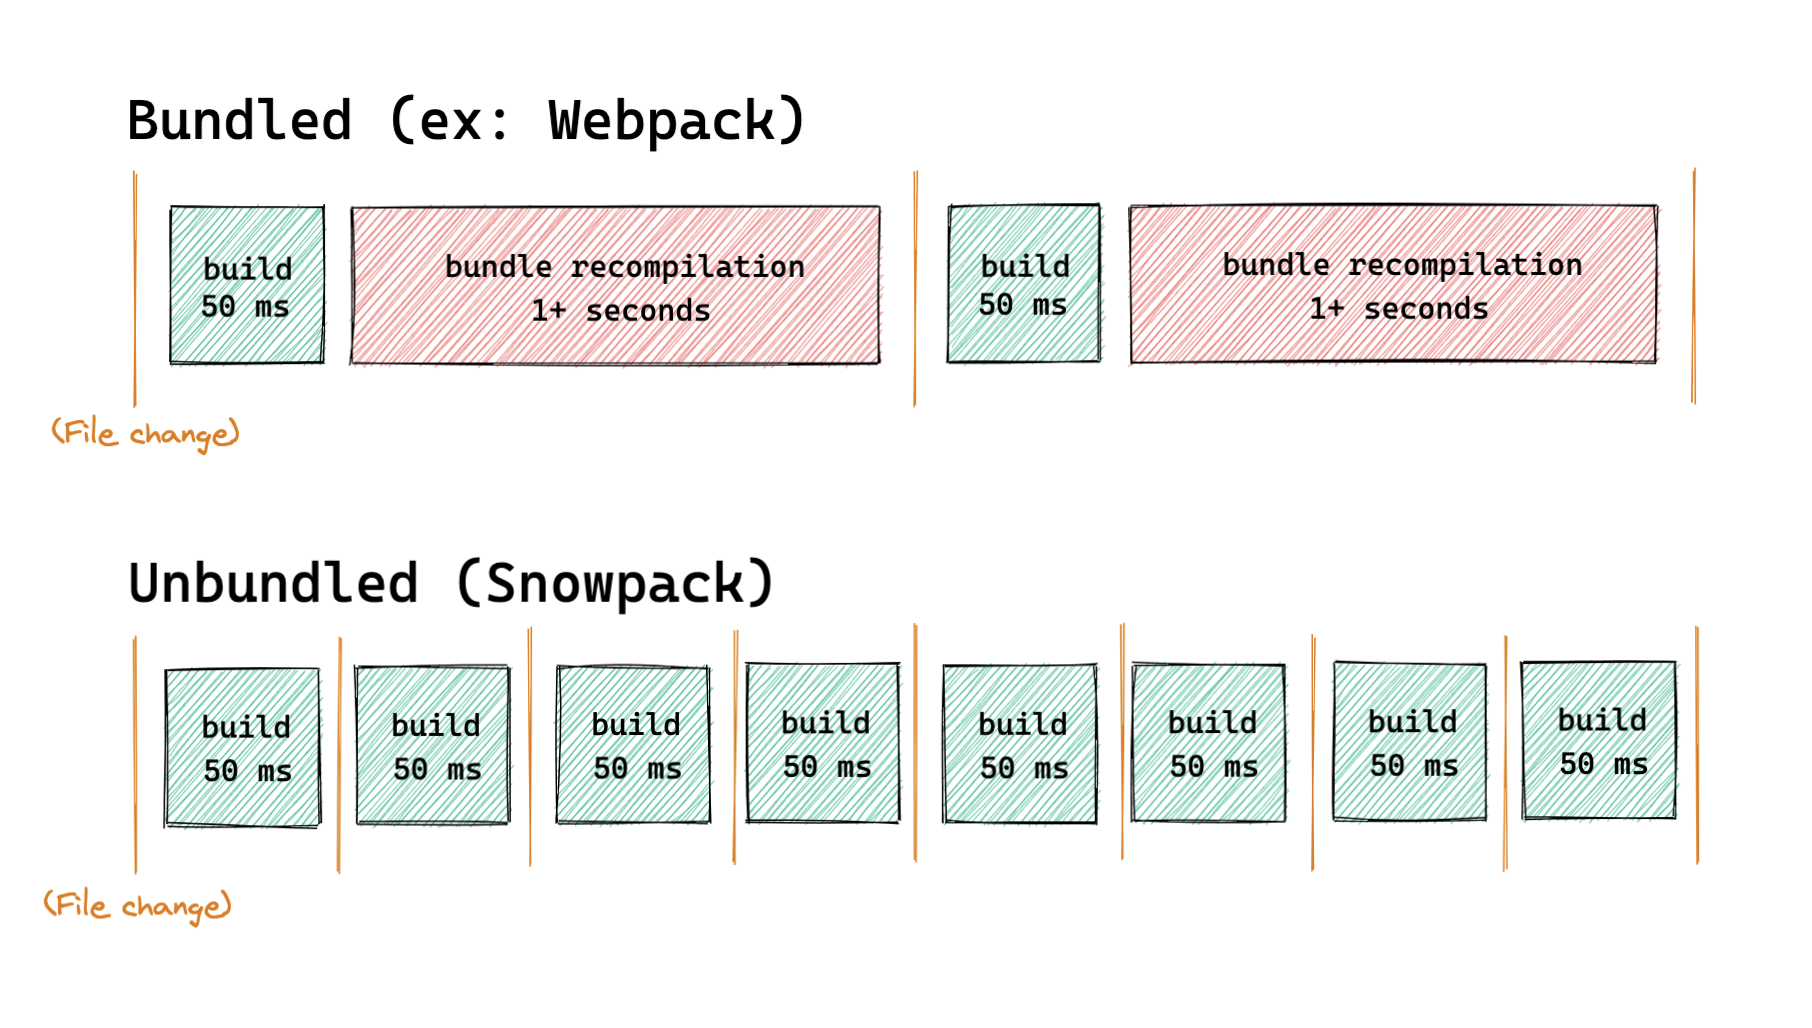
\includegraphics[scale=0.5]{Bundledvsunbundled}
   \caption{Gebundeld vs ongebundeld \autocite{snowpack-no-date}}
\end{figure}

Dit alles resulteert in zeer snelle prestaties in vergelijking met module bundlers zoals Webpack. Dit alles betekent echter niet dat module bundlers voorbijgestreefd zijn. Sterker nog: ongebundelde build tools gebruiken ook module bundlers, de ene al meer dan de ander. Dit wordt gedaan omdat de voordelen van Tree-shaking, een enkel uitvoerbestand en andere pluspunten van module bundlers nog steeds gelden. In hoofdstuk 3 zal hier dieper op ingegaan worden.

Voor de rest van deze proef zal de verzamelnaam “build tools” gebruikt worden om naar module bundlers en ongebundelde build tools te verwijzen. Module bundlers zijn namelijk ook tools die een webapplicatie helpen builden, maar dan gebundeld. Waar mogelijk zal natuurlijk de meest specifieke term gebruikt worden.

\subsection{Keuze build tools}

In deze paragraaf zullen voorbeelden van build tools worden besproken. Eerst twee module bundlers, daarna twee ongebundelde build tools. Vooral in de categorie van module bundlers zijn er veel meer voorbeelden te vinden (Rollup, Fusebox, Browserify, …), hoewel ze allemaal hetzelfde resultaat willen bekomen: een gebundelde webapplicatie aan een browser kunnen leveren. Aangezien de verschillen tussen de meeste helemaal niet groot zijn, is het vrij nutteloos een hele requirement analyse op te bouwen. De twee keuzes voor de module bundler categorie werden gemaakt aan de hand van populariteit en hoe veel ze van elkaar verschillen. De zoektocht naar ongebundelde build tools voor deze proef was een pak gemakkelijker. Er zijn er namelijk maar twee met een deftige user-base. 

Hoewel de modernere aanpak van ongebundelde build tools in opmars is, zijn module bundlers zeker nog niet voorbijgestreefd. De verschillen en voorbeelden zullen worden uitgelegd in de volgende sectie. 

\subsubsection{Webpack}

Webpack is de meest populaire module bundler in de wereld \autocite{}. Dit heeft veel te maken met het feit dat het één van de oudste is. Het wordt voorgeïnstalleerd in veel \gls{web frameworks} zoals create-react-app en Next.js \autocite{}. Op deze manier wordt het door velen gebruikt zonder dat ze het weten. Het wordt geleverd met een optionele ingebouwde ontwikkelserver die het opzetten van een lokale ontwikkelomgeving eenvoudiger maakt.

Webpack draait op Node.js. Het kan zijn werk doen zonder enige configuratie, maar is zeer configureerbaar indien nodig. Het ondersteunt de hierboven besproken module types en meer. Omdat Webpack standaard alleen Javascript en JSON bestanden begrijpt, worden Loaders gebruikt om de verwerking van andere bestandstypen mogelijk te maken door ze om te zetten in geldige modules. Met behulp van Loaders kunnen andere typen modules of zelfs assets zoals afbeeldingen worden geïmporteerd en verwerkt door Webpack. Bovendien kan Webpack ook worden uitgebreid met plugins. Deze maken een brede waaier aan extra functionaliteit mogelijk, zoals bundel optimalisatie. 

De functie van een module bundler is al besproken. Maar hoe bereikt Webpack dit? Wanneer een bestand afhankelijk is van een ander in een project, ziet Webpack dat en zet in zijn dependency graph.

\begin{figure}[h]
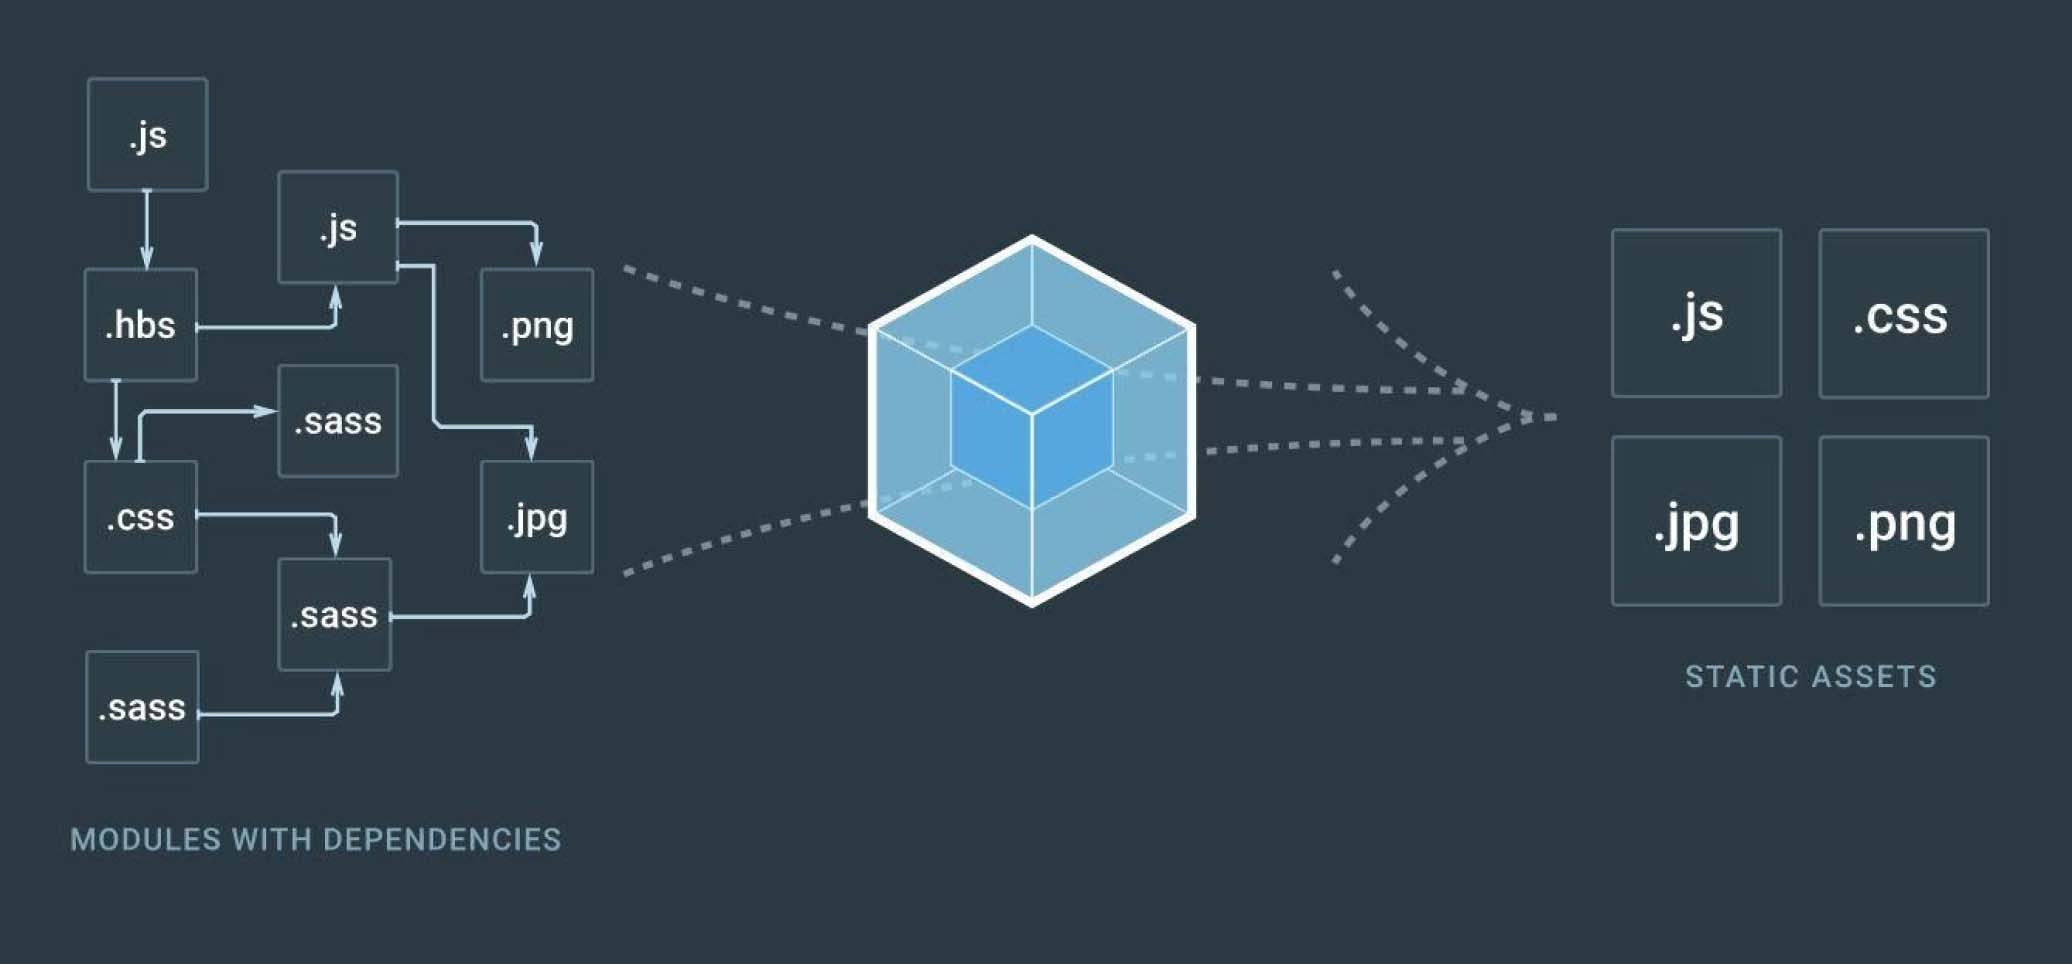
\includegraphics[scale=0.9]{Webpack}
   \caption{Essentiele functie module bundler \autocite{webpack-no-date}}
\end{figure}

Deze graaf wordt recursief opgebouwd. Wanneer het tijd is om de applicatie te bouwen, gebruikt het de dependency graph om alle bestanden samen te voegen tot één uitvoerbestand dat dan naar de browser wordt verzonden. Module bundlers en dus Webpack ook doen dit zowel in ontwikkeling als in productie.

\subsubsection{Parcel}

Parcel is een andere module bundler. Het draait echter niet op Node.js, in plaats daarvan is de compiler die het gebruikt gebouwd met Rust. Rust is een gecompileerde programmeertaal. Zonder al te veel in detail te treden, betekent dit dat Rust code direct naar machine code wordt gecompileerd, wat resulteert in snellere prestaties. Het doet veel van dezelfde dingen die Webpack doet zonder enige configuratie. Toen het werd uitgebracht, was het belangrijkste kenmerk dat het geen configuratiebestand nodig had en Webpack wel. Nu kan Webpack echter ook zijn werk doen zonder een configuratiebestand. Hoewel een no-configuratie aanpak geweldig is voor kleinere projecten, is het vaak niet haalbaar voor een grote applicatie. 

\subsubsection{Snowpack}

Snowpack is het eerste voorbeeld van een ongebundelde build tool. Het is momenteel de meest populaire in zijn categorie. Het pakt uit met de slogan ‘The faster build tool’. Of dat effectief waar is, zal in het volgend hoofdstuk besproken worden. Het grootste pluspunt van Parcel was dat die zijn doel probeert te bereiken met zo min mogelijk configuratie. Deze filosophie volgt Snowpack niet. Een configuratie bestand is vereist en kan al snel aanzienlijke grootte bereiken.

Zoals hierboven vermeldt, gebruikt een build tool vaak toch een module bundler in productie. Bij Snowpack is dit echter optioneel. Standaard is de productie build die Snowpack aanmaakt dus ook ongebundeld, iets waar enkel moderne browsers mee overweg kunnen. De configuratie kan wel aangepast worden om gebruik te maken van Webpack of Rollup, nog een andere module bundler, zodat dat laatste geen probleem meer vormt. Voor dit onderzoek voegen we zo’n module bundler niet toe aan Snowpack. Bij de volgende build tool die aan bod komt, Vite, is het geen optie om de module bundler in productie weg te laten. Snowpack zal dus de volledige ongebundelde applicatie representeren, terwijl Vite hetzelfde zal doen voor half-ongebundelde.

\subsubsection{Vite}
Vite is de jongste build tool die in deze studie aan bod komt. Het combineert een ongebundelde development omgeving met een gebundelde in productie. Voor dit laatste gebruikt het Rollup \autocite{vite-no-date}, een alternatief van Webpack. Hoewel het ook een configuratie bestand bevat, is die veel minder groot en ingewikkeld dan Snowpack.

Zoals de naam Vite doet vermoeden, beweren de makers ervan bliksemsnelle opstart- en buildtijden in vergelijking met de competitie.


In de twee volgende hoofdstukken zullen de besproken build tools getest en vergeleken worden. Eerst bij het opzetten van een nieuw project en daarna bij het omvormen van een bestaand. Elk hoofdstuk bevat een eigen conclusie, als laatste volgt de algemene.

